% mnras_template.tex 
%
% LaTeX template for creating an MNRAS paper
%
% v3.0 released 14 May 2015
% (version numbers match those of mnras.cls)
%
% Copyright (C) Royal Astronomical Society 2015
% Authors:
% Keith T. Smith (Royal Astronomical Society)

% Change log
%
% v3.0 May 2015
%    Renamed to match the new package name
%    Version number matches mnras.cls
%    A few minor tweaks to wording
% v1.0 September 2013
%    Beta testing only - never publicly released
%    First version: a simple (ish) template for creating an MNRAS paper

%%%%%%%%%%%%%%%%%%%%%%%%%%%%%%%%%%%%%%%%%%%%%%%%%%
% Basic setup. Most papers should leave these options alone.
\documentclass[fleqn,usenatbib]{mnras}

% MNRAS is set in Times font. If you don't have this installed (most LaTeX
% installations will be fine) or prefer the old Computer Modern fonts, comment
% out the following line
\usepackage{newtxtext,newtxmath}
% Depending on your LaTeX fonts installation, you might get better results with one of these:
%\usepackage{mathptmx}
%\usepackage{txfonts}

% Use vector fonts, so it zooms properly in on-screen viewing software
% Don't change these lines unless you know what you are doing
\usepackage[T1]{fontenc}

% Allow "Thomas van Noord" and "Simon de Laguarde" and alike to be sorted by "N" and "L" etc. in the bibliography.
% Write the name in the bibliography as "\VAN{Noord}{Van}{van} Noord, Thomas"
\DeclareRobustCommand{\VAN}[3]{#2}
\let\VANthebibliography\thebibliography
\def\thebibliography{\DeclareRobustCommand{\VAN}[3]{##3}\VANthebibliography}


%%%%% AUTHORS - PLACE YOUR OWN PACKAGES HERE %%%%%

% Only include extra packages if you really need them. Common packages are:
\usepackage{graphicx}	% Including figure files
\usepackage{amsmath}	% Advanced maths commands
\usepackage{amssymb}	% Extra maths symbols

%%%%%%%%%%%%%%%%%%%%%%%%%%%%%%%%%%%%%%%%%%%%%%%%%%

%%%%% AUTHORS - PLACE YOUR OWN COMMANDS HERE %%%%%

% Please keep new commands to a minimum, and use \newcommand not \def to avoid
% overwriting existing commands. Example:
%\newcommand{\pcm}{\,cm$^{-2}$}	% per cm-squared

%%%%%%%%%%%%%%%%%%%%%%%%%%%%%%%%%%%%%%%%%%%%%%%%%%

%%%%%%%%%%%%%%%%%%% TITLE PAGE %%%%%%%%%%%%%%%%%%%

% Title of the paper, and the short title which is used in the headers.
% Keep the title short and informative.
\title[DES SN Ia Galactic Rate]{Supernova Host Galaxies in the Dark Energy Survey: III. The Evolving Galactic Rate of Type Ia Supernovae}

% The list of authors, and the short list which is used in the headers.
% If you need two or more lines of authors, add an extra line using \newauthor
\author[P. Wiseman et al.]{
P. Wiseman,$^{1}$\thanks{E-mail: p.s.wiseman@soton.ac.uk}
A. N. Other,$^{2}$
Third Author$^{2,3}$
and Fourth Author$^{3}$
\\
}

% These dates will be filled out by the publisher
\date{Accepted XXX. Received YYY; in original form ZZZ}

% Enter the current year, for the copyright statements etc.
\pubyear{2020}

% Don't change these lines
\begin{document}
\label{firstpage}
\pagerange{\pageref{firstpage}--\pageref{lastpage}}
\maketitle

% Abstract of the paper
\begin{abstract}
This is a simple template for authors to write new MNRAS papers.
The abstract should briefly describe the aims, methods, and main results of the paper.
It should be a single paragraph not more than 250 words (200 words for Letters).
No references should appear in the abstract.
\end{abstract}

% Select between one and six entries from the list of approved keywords.
% Don't make up new ones.
\begin{keywords}
keyword1 -- keyword2 -- keyword3
\end{keywords}

%%%%%%%%%%%%%%%%%%%%%%%%%%%%%%%%%%%%%%%%%%%%%%%%%%

%%%%%%%%%%%%%%%%% BODY OF PAPER %%%%%%%%%%%%%%%%%%

\section{Introduction}

Type Ia supernovae (SNe Ia) are explosions of white dwarves (WDs) at masses close to the Chandrasekhar limit of 1.44 $M_{\odot}$. The small observed dispersion in their peak brightnesses can be reduced further through empirical relations between brightness and light curve properties, such as decline rate (stretch) or optical colour. These properties have led SNe Ia to be used extensively by cosmologists to measure relative distances in the Universe.

Despite reducing dispersions to $\sim 0.1$ mag in samples with over one thousand SNe \citep{Scolnic2018}, the exact nature of the progenitor scenarios for SNe Ia is yet to be confirmed. While it is accepted that SNe Ia are caused by accretion of matter onto a WD from a companion star, multiple possible scenarios exist for the nature of that companion star and the search for this has formed a significant field of research (see \citealt{Maoz2014} for a review). The leading models involve a main sequence (MS) star in the single-degenerate (SD) scenario \citep{Whelan1973,Nomoto1982}, a secondary white dwarf in the double-degenerate (DD) scenario \citep{Tutukov1976,Iben1984,Webbink1984}, while more exotic models such as the core-degenerate (CD) scenario invoke white dwarves merging with the cores of massive stars \citep{Soker2019}. 

The progenitors of a number of core-collapse SNe (CCSNe) have been identified in high-resolution pre-explosion images, allowing detailed analysis of the latter stages of massive star evolution. However, this approach has not yet been successful in identifying a progenitor of a SN Ia. Conversely, it has been possible to search for surviving remnants of the binary system -- main sequence stars or white dwarves left behind at the SN location or kicked \citep{Shen2018} -- displaying tentative evidence for a DD scenario. As yet, there is no conclusive evidence ruling out any progenitor channel from being a significant contribution to the total population of SNe Ia.

Another method of inferring progenitor channels is the study of the SN Ia delay time distribution (DTD). The DTD can be interpreted as the rate at which SNe Ia occur as a function of the delay time $\tau$ since an episode of star-formation, and thus carries characteristic signatures of the progenitor channel (see \citealt{Wang2012} for a review). While the SD scenario is able to produce a broad range of functional forms of the DTD, the DD scenario predicts a power law of the form $t^{\beta}$, with $\beta \sim -1$ \citep[e.g][]{Ruiter2009,Mennekens2010}.

Given the vast range of timescales to which the DTD is sensitive, it is non-trivial to measure and various techniques have been developed to infer it indirectly. One such approach is to measure global properties of SN Ia host galaxies. Simple examples of such analyses are comparisons of the rates of SNe Ia in hosts that have been split by some observational property, such as morphology or colour, and have shown that SNe Ia rate per unit stellar mass (SNuM) is significantly larger in late-type spiral galaxies as well as in bluer galaxies \citep[e.g.][]{Mannucci2005}. These observations heavily imply that SNe Ia rates are dependent on recent or ongoing star-formation, and thus that the majority of SNe Ia explode after short delay times. Conversely, the SNuM in E/S0 and red galaxies is non-negligible, suggesting that there is a secondary, much older component to the DTD \citep{Sullivan2006,Smith2012}. The DTD is thus approximated by a two-component ("$A + B$") model, where $A$ and $B$ are the normalizations of the DTD for "prompt" (i.e. proportional to instantaneous SFR) and "tardy" (i.e. proportional to overall stellar mass) SNe, respectively A complementary technique involves measuring the evolution of the volumetric rate of SNe Ia as a function of redshift and comparing this evolution to the average cosmic star-formation history (CSFH) of the Universe \citep{Gal-Yam2004,Strolger2004,Dahlen2004,Dahlen2008}. This technique is also applicable to galaxy clusters, for which it is assumed that the star-formation histories are strongly peaked at some past epoch and thus that the rate of SNe Ia in clsuters as a function of redshift is a more direct measure of the DTD \citep{Maoz2004,Graur2014,Maoz2014}. Conversely, it is also possible to estimate the SFH of an individual galaxy through the modelling of its stellar populations via spectral energy distribution (SED) fitting. Works such as \citet{Maoz2011}, \citet{Maoz2012}, \citet{Graur2013} estimated the DTD by measuring SFHs for a sample of field galaxies and comparing them to the number of SNe detected in each galaxy. and has led to results that suggest a DTD power law with $\beta$ consistent with $-1$ \citep[e.g.][]{Maoz2011,Graur2013}. \citet{Childress2014} showed that the $A+B$ parameterisation arises as a direct consequence of the combination of a power-law DTD with the SFHs of galaxies.

In this work, we combine parts of the above methods and derive a new, independent measurement of the SN Ia DTD. Instead of measuring the volumetric rate of SNe Ia, we measure the rate per galaxy as a function of stellar mass, as per \citet{Sullivan2006,Smith2012}. We use the stellar mass assembly model of \citet{Childress2014} to predict the stellar age distribution of galaxies for a given stellar mass at the mean redshift of our SN sample, and then forward model the DTD by convolving it with the stellar age distribution and comparing the predicted rates to the observed rates.




\section{Method \label{sec:method}}

We represent the SN Ia DTD by a power law of the form:

\begin{equation}
    \Phi(\tau) = A\left(\frac{\tau}{\mathrm{Gyr}}\right)^{\beta}\,,
\end{equation} 
where $\tau$ is the time since a burst of star formation, and $A$ is a normalisation at $\tau=1\mathrm{Gyr}$. If all stars in a galaxy were formed at a single epoch $t_f$, the DTD would describe the rate of SNe at an observation time $\tau = t_0$. However in reality galaxies are formed by the gradual build up of stellar mass over several epochs of star formation -- the distribution of this mass build up is known as the star-formation history (SFH). The rate of SNe Ia is thus the sum of the DTD evaluated for each epoch of star formation, multiplied by the stellar mass formed in that epoch. Mathematically this is represented by the convolution of the DTD and SFH:
 
 
\begin{equation}
    R_{\mathrm{G}} = \int_{t_0}^{\infty} \psi(t_0-\tau)\Phi(\tau)\,d\tau \,,
\end{equation}
where $t_0$ is the epoch at which the galaxy is observed, and $\psi$ is the SFH.

\subsection{Modeling the star formation histories of galaxies \label{subsec:method_sfh}}
To model the SFH of galaxies as a function of their stellar mass we adopt the model of \citet{Childress2014}. In the model, galaxies are expected to evolve smoothly along the so-called "main sequence of star formation" whereby the SFR of a galaxy of stellar mass $M_*$ at redshift $z$ is determined by a simple relationship (the SMz relation, \citealt{Zahid2012}). Specifically, we implement their "fine-tuned" model (C14 Eq. A7), whereby the SMz flattens above $z\sim2$ in line with observations \citep{Stark2013}. We adjust this model slightly and arrive at a final SMz:

\begin{equation}
    \Psi(M_*,z) = \left(\frac{M_*}{10^{10}}\right)^{0.7}\frac{\exp{\left(1.9z\right)}}{\exp{\left(1.7\left(z-2\right)\right)} + \exp{\left(0.2\left(z-2\right)\right)} } [\mathrm{M}_{\odot} \mathrm{yr}^{-1}]\,.
\end{equation}

As galaxies grow, their SFR begins to slow down and eventually shut off almost entirely in a process known as quenching. We adopt the quenching penalty $p_Q$ directly from \citet{Childress2014}:
\begin{equation}
    p_Q(M_*,z) = \frac{1}{2}\left[1 - \mathrm{erf}\left(\frac{\log(M_*) - \log(M_Q(z)}{\sigma_Q}\right)\right]\,,
\end{equation}
where $M_Q(z)$ describes how the quenching mass evolves with redshift, and $\sigma_Q$ is the transition scale which controls how fast a galaxy quenches. We adopt the observationally motivated form of the quenching mass evolution (Eq. A8 from \citealt{Childress2014}):
\begin{equation}
    \log(M_q(z)/\mathrm{M}_{\odot}) = 10.077 + 0.636z \,, 
\end{equation}
and a transition scale of $\sigma_Q = 1.1$. 

As per \citet{Childress2014} we plant seed galaxies with initial masses of $10^6 \mathrm{M}_{\odot}$ at intervals of 50 Myr for look-back times $1 \leq t_f \leq 10$ Gyr, and 25 Myr for look-back times $10 \leq t_f \leq 13$ Gyr, and evaluate the model with a time step of 0.5 Myr.

The rate of SNe per galaxy ($R_{\mathrm{G}}$) per year in a transient survey can be approximated by the simple equation:
\begin{equation}
    R_{\mathrm{G}} = \frac{N_{\mathrm{SN}}}{N_{\mathrm{G}}} \frac{A_{\mathrm{G}}}{A_{\mathrm{SN}}} \frac{1}{T_{\mathrm{SN  survey}}}\,,
\label{eq:rate1}
\end{equation}
where $N_{\mathrm{SN}}$ and $N_{\mathrm{G}}$ are the respective number of SNe and galaxies detected, $A_{\mathrm{SN}}$ and $A_{\mathrm{G}}$ the sky areas from which the SNe and G samples were taken, and $T$ the duration of the SN survey in years. By binning both the SN hosts and field galaxies by their stellar mass we can approximate the function $R_{\mathrm{G}}(M_*)$.

\begin{table}
	\centering
	\caption{Numbers of field galaxies and SN hosts passing various quality cuts.}
	\label{tab:field_vuts}
	\begin{tabular}{lccr} % four columns, alignment for each
		\hline
		Cut & N (galaxies, X3)  & N (SN hosts)\\
		\hline
		Chosen fields & 1364311  & 1766\\
	    Kron mag in all bands & 1069004  & 1764 \\
	    Masked chips & 816950  & - \\
	    Has ugrizJHK photometry & 545748  & -\\
	    Edge of chip & 481731 & 1716 \\
	    Star/galaxy separation & 400051 &  1678\\
	    Has good redshift & 395034 & 1678 \\
	    SNR $\geq 3$& 338256  & 1678 \\
	    $m_r \leq 26.5$ & 196109 &  1678 \\
	    $0.2 \leq z \leq 0.8$ & 48177 & 1414\\ 
	    
		\hline
	\end{tabular}
\end{table}

\section{Data \label{sec:data}}
\subsection{Dark Energy Survey supernova programme \label{subsec:des}}
The DES Supernova Programme (DES-SN) is a transient survey based on five six-month seasons of observations with the Dark Energy Camera (DECam; \citealt{Flaugher2015}), designed primarily to measure the light curves of SNe Ia for use as cosmological distance indicators. Transients were detected and processed using a difference imaging program \citep{Kessler2015} and vetted using a machine learning (ML) algorithm \citep{Goldstein2015}. Spectral follow-up was performed on a suite of large optical telescopes \citet{Smith2020b}, leading to the initial publication of a measurement of cosmological parameters using 207 spectroscopically confirmed SNe (\citealt{DESCollaboration2018a}, and references therein). 
\subsection{Supernovae \label{subsec:host_sample}}
\subsubsection{Photometric classification and quality cuts \label{subsubsec:sn_classify}}
With over 30,000 transients passing ML cuts it was not possible to obtain spectral follow up of every object. Instead we make use of photometric classification techniques, in particular the recurrent neural network \texttt{superNNova} (SNN; \citealt{Moller2019}). We derive our SN Ia sample following the approach of \citet{Scolnic2020}, but use a threshold probability of $P(\mathrm{Ia})\geq0.5)$. The photometricially classified SNe Ia are then passed through the \texttt{SALT2} framework \citep{Betoule2014} and are subject to quality cuts on the light curve width (stretch; $x_1$) and colour ($c$) parameters: $-3 \leq x_1 \leq 3$, $-0.3 \leq c \leq 0.3$. These cuts help to reduce the potential contamination from core-collapse SNe (CCSNe) and outlying SNe Ia whose physical mechanisms may diverge from the general cosmologically useful population.

\subsubsection{Host galaxy selection \label{subsubsec:sn_hosts}}
Host galaxies for all transients in DES-SN are derived from the deep-stacked $g, r, i, z$-band images presented in \citet{Wiseman2020}. SN are associated to hosts using the directional light radius method \citep[e.g.][]{Sullivan2006,Gupta2016}, while spectroscopic redshifts are provided by OzDES \citep{Yuan2015,Childress2017,Lidman2020}, leading to an initial sample of 1766 SNe.

\subsection{Field galaxies\label{subsec:field_sample}}
A sample of field galaxies is obtained from the same catalogue to which the SNe are matched to obtain host galaxies, and is presented in a companion paper \citet{Wiseman2021}. The steps relevant to this analysis are outlined in the following sections.

\subsubsection{Photometric redshifts \label{subsubsec:photozs}}


Since the vast majority of objects in the \citet{Wiseman2021} catalogue do not have a spectroscopic redshift measurement, we rely on photometric redshifts (photo-$z$s) in order to proceed with the analysis. 
Photometric redshifts are taken, where available, from the catalogue of \citet{Hartley2020}, and have been estimated using the \texttt{EAZY} photometric redshift code \citep{Brammer2008}. These photo-$z$s make use of deep DES optical photometry alongside DECam $u$-band data and near-infrared (NIR) $J$, $H$, and $K$-band imaging from the ultraVISTA and VIDEO surveys. 

\subsubsection{Galaxy properties \label{subsubsec:properties}}

We estimate global galaxy properties for both the SN host and field galaxy samples by fitting the photometry with stellar population templates in a method outlined by \citet{Sullivan2006} and consistent to that used in previous DES-SN analyses \citep{Kelsey2020,Smith2020,Wiseman2020}. For SN hosts the redshift is fixed at the spectroscopically determined value, while for field galaxies we fix it at either the spectroscopic value if one exists (a minority of cases), or more commonly the photometrically derived value. The fitting procedure returns a best fitting template and corresponding stellar mass ($M_*$) and SFR averaged over the proceeding 250 Myr. Uncertainties on the properties are estimated by refitting the templates to the photometry that has been resampled from Gaussian PDFs formed by the photometric fluxes and their uncertainties. 

\subsection{Quality cuts \label{subsec:cuts}}

In order to refine the sample of host and field galaxies for the rate analysis we perform a series of quality cuts. Firstly, we require that a galaxy must be detected and have a Kron magnitude measurement in all four DES optical bands. We also require that it is not within a given number of pixels of the CCD edge, as the co-addition of slightly misaligned images introduced a region of significant noise in this part of the detector. To remove high-probability stellar sources we apply a cut of 0.95 in the star/galaxy (S/G) separation \texttt{CLASS\_STAR} provided by \texttt{Source Extractor} \citep{Bertin1996}. 

\begin{figure}
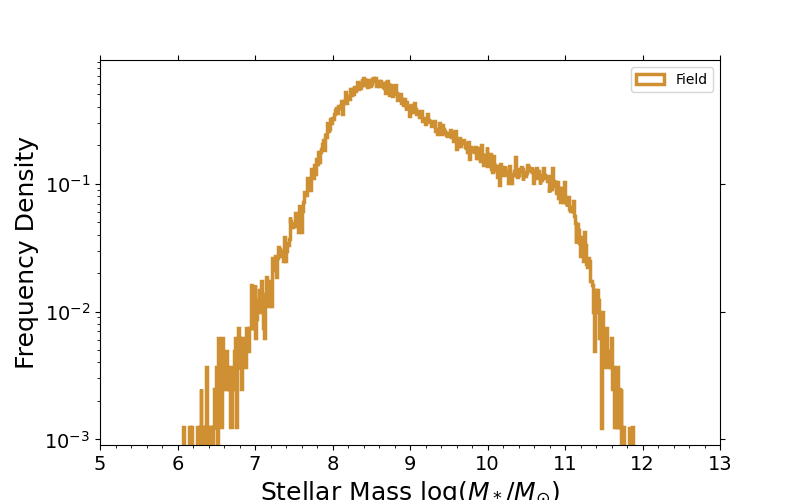
\includegraphics[width=0.5\textwidth]{figs/mass_hist_log.png}
\caption{Distribution of the stellar mass of the field galaxies used in the analysis. The distribution is well desribed by a Schechter function.
\label{fig:log_mass_field}}
\end{figure}


\section{Incompleteness corrections \label{sec:incompleteness}}

Although Eq. \ref{eq:rate1} serves as an approximation to the SN rate per galaxy per year, both the SN and field galaxy samples introduced in Sections \ref{subsec:host_sample} and \ref{subsec:field_sample} are affected by incompleteness, which is likely to be the dominant systematic effect in the analysis. In this section we describe our method of correcting for various sources incompleteness in the data.

\subsection{Supernovae \label{subsec:incompleteness_SNe}}

Incompleteness in a SN survey arises from a number of sources. The primary source of incompleteness is caused by the magnitude limit of the survey: SNe with apparent magnitudes below the survey limit will not be detected. Since SNe Ia are relatively uniform in absolute luminosity, this form of incompleteness is primarily redshift dependent. On the other hand, DES-SN comprises 10 separate pointings, each with different visibility and thus airmass throughout the observing season. These differences lead to different detection efficiencies across the fields.

To correct for these incompleteness, we follow a similar method to that used in the PTF rates analyses of \citet{Frohmaier2019,Frohmaier2020} as well as the DES-SN superluminous SN rate of \citet{Thomas2020}. We run a suite of simulations using \texttt{SNANA} \citet{Kessler2009a}. We simulate 230,000 SNe in the redshift range $0.05 \leq z_{\mathrm{SN}} \leq 1.3$, and draw peak magnitudes from \textbf{ADD DETAILS}. We then run mock versions of the DES-SN survey, using the exact cadence, conditions, and zeropoints from the survey itself. All of the detected simulated SNe are passed through the light curve fit of SALT2 \citep{Betoule2014}, as per the implementation in \texttt{SNANA}, and those that fail the light curve cuts outlined in Section \ref{subsubsec:sn_classify} are discarded. We are left with a fraction of the original simulated SNe, and that fraction is dependent on location, explosion epoch, and redshift, which we define as the SN efficiency. For the $i$th SN the efficiency $\eta_{\mathrm{SN}, i}$ in field $F$, exploding at time $t_0$ at redshift $z$, is:
\begin{equation}
    \eta_{\mathrm{SN},i} (F_i,z_i,t_{0,i}) = \left( \frac{N_{\mathrm{obs}}\left(F_i,z_i,t_{0,i}\right)}{N_{\mathrm{sim}}\left(F_i,z_i,t_{0,i}\right)}\right)\,.
\end{equation}

The distribution of efficiency as a function of redshift is shown in Figure \ref{fig:efficiencies}. It is evident that the deep fields (X3, C3) are sensitive to SNe at higher redshifts, while there is no drastic shifts between efficiencies in the eight shallow fields. 


\subsection{Supernova hosts \label{subsec:incompletenss_SN_hosts}}
A further limiting factor in the SN host sample is the requirement of a spectroscopic redshift. The majority of SN host spectroscopic redshifts in DES are provided by the dedicated follow-up survey OzDES, for which the limiting magnitude is around 24 to 24.5 mag in the $r$ band. The rate at which a host redshift is successfully measured given an apparent magnitude has been extensively modelled by \citetalias{V20} who provide the spectroscopic redshift efficiency as a function of host $r$-band magnitude, host galaxy colour, and the year in which the SN was discovered in order to allow for a longer possible spectroscopic exposure time for hosts of SNe discovered earlier in the survey. So that we reduce any bias towards SNe in bright hosts that are easier to obtain spectroscopic redshifts for, we assign each SN in the sample described in Section \ref{subsec:host_sample} a weight equal to the inverse of the spectroscopic efficiency for its host. This is equivalent to assuming that an efficiency of 0.1 means that for every ten SNe with hosts at that magnitude, only 1 will make it into the sample.

\subsection{Field galaxies \label{subsec:incompleteness_field}}

\subsubsection{Apparent magnitude limits \label{subsubsec:mag_lims}}
As we use photometric, rather than spectroscopic, redshifts for the field galaxies, they do not suffer from spectroscopic incompleteness as the SN hosts do. Instead, the inclusion of any given galaxy in the survey area in the sample is determined simply by whether it is detected above a prescribed threshold in signal-to-noise ratio, i.e. the sample is magnitude limited. To determine the apparent magnitude limit in each of the optical bands we employ the method of \citet{Johnston2007,Teodoro2010,Johnston2012} (hereafter Completeness I, II, III respectively). Test statistics $T_C$ and $T_V$ are computed based on absolute magnitude and distance modulus by calculating the rank of each galaxy's absolute magnitude (distance modulus) when compared to all other galaxies in a survey within a certain slice of distance modulus (absolute magnitude). For a galaxy of apparent magnitude $m < m_{\mathrm{lim, trial}}$ observed in a survey complete to magnitude $m_{\mathrm{lim, true}}$ where  $m_{\mathrm{lim, trial}} \leq m_{\mathrm{lim, true}}$, the expectation value of the rank is 0.5. However, if a trial limiting magnitude $m_{\mathrm{lim, trial}} \geq m_{\mathrm{lim, true}}$, there will be a lack of observed faint objects, such that the expectation value of the rank drops. Completeness I, II, and III show that for surveys with sharp, well defined magnitude limits the test statistics $T_C$ and $T_V$ drop sharply. The DES deep stacks present a more challenging case. They cover a wide area and are compiled from tens of separate CCDs, each with its own detection efficiency. Moreover, galaxy redshifts have been estimated using photometry only, and $K$-corrections performed using an imperfect template fit, potentially leading to large systematic and statistical fluctuations in absolute magnitudes and distance moduli. To reduce the inhomogeneity while still including  large sample of objects, we split the sample into the deep (X3) and shallow (E2) fields and calculate limiting magnitudes separately. Figs. \ref{fig:completeness_X3, fig:completenessE2} show the values of $T_C$ and $T_V$ for the two fields respectively. The values of the test statistics increase with $m_{\mathrm{lim, trial}}$ until a peak, before decreasing to stable values at magnitudes far beyond the limit of the survey. The shape at brighter $m_{\mathrm{lim, trial}}$ is likely caused by incompleteness at the bright end: due to the small sky area, we simply do not probe enough volume to sample the bright end of the galaxy luminosity function well enough for the statistics to be robust. To approximate an efficiency function, we fit the peak of the statistics with a polynomial function, and then normalise by the maximum and minimum values. We then interpolate between the peak and the faint-magnitude floor to find the 50\% completeness limit at the point where the normalised value of the test statistic is 0.5. These values are consistent with the value at which 50\% of the true sources are detected but have the advantage of being derived from the data without a simulation that is based on assumptions and thus susceptible to bias.

\subsubsection{$V_{\mathrm{max}}$ correction \label{subsubsec:vmax_corr}}

To correct for incompleteness caused by the magnitude limited nature of the survey we follow the prescription of e.g. \citet{Sullivan2006, Smith2012} by using a $V_{\mathrm{max}}$ method of \citet{Schmid1968}. For each galaxy in the sample we calculate the maximum volume within which it would have been observed given its absolute magnitude and $k-$correction. A correction of $V_{\mathrm{survey}}/V_{\mathrm{max}}$ is applied to all galaxies for which $V_{\mathrm{max}} < V_{\mathrm{survey}}$, where $V_{\mathrm{survey}}$ is the maximum volume reached by the survey. In our case this corresponds to the volume at $z=0.8$. Figs. \ref{fig:vmax_gals} and \ref{fig:vmax_hist} show the distribution of the correction among galaxies in the sample. The vast majority of galaxies require no correction, meaning they would have been observed beyond the maximum volume considered. Roughly 1\% of objects have a correction greater than 1, with the distribution well described by a power-law function. In Section \ref{sec:rates} we split the samples into redshift bins in order to measure cosmic evolution of the SN Ia rate. For each redshift bin, we reevaluate the value of $V_{\mathrm{survey}}$ used in the incompleteness correction to be the volume of the bin.

\section{Rates as a function of host galaxy properties \label{sec:rates}}

\subsection{Dependence of the SN Ia rate on stellar mass \label{subsec:rates_mass}}

\subsection{Dependence of the SN Ia rate on SFR \label{subsec:rates_sfr}}

\section{Conclusions}

The last numbered section should briefly summarise what has been done, and describe
the final conclusions which the authors draw from their work.

\section*{Acknowledgements}

The Acknowledgements section is not numbered. Here you can thank helpful
colleagues, acknowledge funding agencies, telescopes and facilities used etc.
Try to keep it short.

%%%%%%%%%%%%%%%%%%%%%%%%%%%%%%%%%%%%%%%%%%%%%%%%%%
\section*{Data Availability}

 
The inclusion of a Data Availability Statement is a requirement for articles published in MNRAS. Data Availability Statements provide a standardised format for readers to understand the availability of data underlying the research results described in the article. The statement may refer to original data generated in the course of the study or to third-party data analysed in the article. The statement should describe and provide means of access, where possible, by linking to the data or providing the required accession numbers for the relevant databases or DOIs.




%%%%%%%%%%%%%%%%%%%% REFERENCES %%%%%%%%%%%%%%%%%%

% The best way to enter references is to use BibTeX:

\bibliographystyle{mnras}
\bibliography{PhilMendeley} % if your bibtex file is called example.bib


% Alternatively you could enter them by hand, like this:
% This method is tedious and prone to error if you have lots of references
%\begin{thebibliography}{99}
%\bibitem[\protect\citeauthoryear{Author}{2012}]{Author2012}
%Author A.~N., 2013, Journal of Improbable Astronomy, 1, 1
%\bibitem[\protect\citeauthoryear{Others}{2013}]{Others2013}
%Others S., 2012, Journal of Interesting Stuff, 17, 198
%\end{thebibliography}

%%%%%%%%%%%%%%%%%%%%%%%%%%%%%%%%%%%%%%%%%%%%%%%%%%

%%%%%%%%%%%%%%%%% APPENDICES %%%%%%%%%%%%%%%%%%%%%

\appendix

\section{Some extra material}

If you want to present additional material which would interrupt the flow of the main paper,
it can be placed in an Appendix which appears after the list of references.

%%%%%%%%%%%%%%%%%%%%%%%%%%%%%%%%%%%%%%%%%%%%%%%%%%


% Don't change these lines
\bsp	% typesetting comment
\label{lastpage}
\end{document}

% End of mnras_template.tex
